\subsection{Unlocking Accuracy: What Impacts Your Frequency Counter?}

\begin{tcolorbox}[colback=gray!10, colframe=black, title=E4B01]
Which of the following factors most affects the accuracy of a frequency counter? 
\begin{enumerate}[label=\Alph*.]
    \item Input attenuator accuracy
    \item \textbf{Time base accuracy}
    \item Decade divider accuracy
    \item Temperature coefficient of the logic
\end{enumerate} \end{tcolorbox}

\subsubsection{Related Concepts}

In order to understand the impact of various factors on the accuracy of a frequency counter, we need to delve into a few electronic and measurement concepts.

1. \textbf{Time Base Accuracy}: The time base of a frequency counter refers to the precision of the time measurement used to determine frequency. A frequency counter measures the number of cycles of a signal in a defined time interval. If the time measurement is inaccurate, the calculated frequency will similarly be inaccurate. This is why time base accuracy is crucial; it directly influences the counter's measurement of frequency.

2. \textbf{Input Attenuator Accuracy}: While it is important, the input attenuator ensures that the signal level is within an acceptable range for the frequency counter's input, but it does not directly affect the frequency measurement's accuracy unless the signal level pushes the system beyond its limits.

3. \textbf{Decade Divider Accuracy}: This component breaks down the frequency of the incoming signal by factors of ten, but it can have a ripple effect on overall accuracy. However, errors introduced by the divider only occur if it is improperly designed or calibrated.

4. \textbf{Temperature Coefficient of the Logic}: This factor also influences frequency counters, but more indirectly, as temperature variations can affect the logic circuitry's performance. Still, this is not the primary factor impacting overall accuracy.

\subsubsection{Conclusion}

After evaluating the factors, we determine that \textbf{Time base accuracy} has the most significant impact on the accuracy of a frequency counter measurement. 

In electronic measurement, it is also crucial to consider precision and calibration of time base generators to ensure that the frequency readings are reliable and valid.

\subsubsection{Diagram}

The following diagram illustrates the components involved in the frequency counter measurement process.

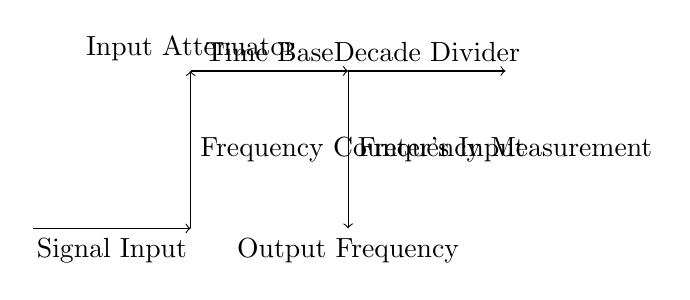
\begin{tikzpicture}
    \draw[->] (0,0) -- (2,0) node[midway,below] {Signal Input} ;
    \draw[->] (2,0) -- (2,2) node[midway,right] {Frequency Counter's Input}
        node[above] {Input Attenuator} ;
    \draw[->] (2,2) -- (4,2) node[midway,above] {Time Base} ;
    \draw[->] (4,2) -- (4,0) node[midway,right] {Frequency Measurement}
        node[below] {Output Frequency} ;
    \draw[->] (4,2) -- (6,2) node[midway,above] {Decade Divider} ;
\end{tikzpicture}
